\textnormal{This project will use various technologies for both the front-end and the back-end. For the back end, we plan to use an SQL database to store the data, as well as Java servlets for code execution. For the front-end, we plan on using Angular and Javascript for the layout and D3.js for the Visual Transcript instances. We may use jQuery for SQL query manipulation that will serve as input to the algorithm that we formulate that will retrieve the necessary data and spawn a Visual Transcript instance on each view.}

\begin{figure}
	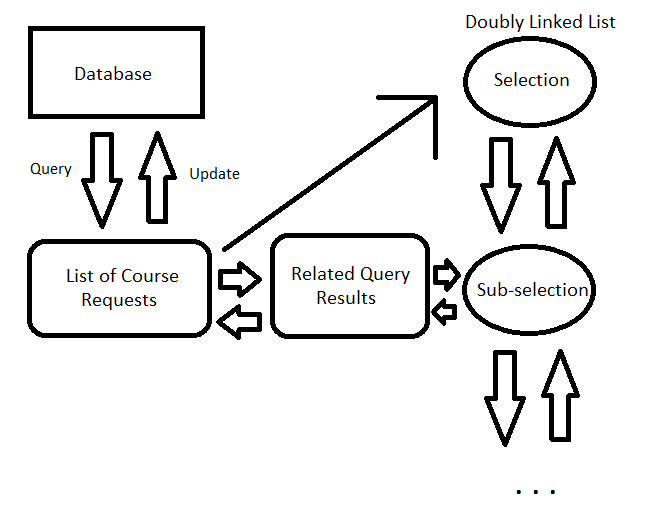
\includegraphics[width=\linewidth]{Data_Structures.png}
	\caption{Internal Data Structures}
	\label{fig:fig1}
\end{figure}

As shown in Figure \ref{fig:fig1}, the backend operations will be primarily driven by queries to the MySQL database. The query results will be fed into the D3.js API that will generate the Visual Transcript visuals. When the user selects certain nodes on the Visual Transcript interface, such as a specific request or a specific class, that item will be stored in a doubly linked list that will allow for progression and regression in the Visual Transcript interface.  Using that linked list will allow our related items retrieval algorithm to populate the Visual Transcript instance with related information regarding the current selection. 
\\\\